% IEEE Transactions on Robotics / Mechatronics Template
\documentclass[letterpaper,journal]{IEEEtran}

% Packages
\usepackage{amsmath,amssymb,amsfonts}
\usepackage{algorithmic}
\usepackage{algorithm}
\usepackage{array}
\usepackage[caption=false,font=normalsize,labelfont=sf,textfont=sf]{subfig}
\usepackage{textcomp}
\usepackage{stfloats}
\usepackage{url}
\usepackage{verbatim}
\usepackage{graphicx}
\usepackage{cite}
\usepackage{xcolor}
\usepackage{booktabs}
\usepackage{multirow}
\usepackage{bm}
% \usepackage[inkscapelatex=false]{svg}

% Figure path
\graphicspath{{figures/}}

% Correct hyphenation
\hyphenation{op-tical net-works semi-conduc-tor IEEE-Xplore}

% ============================================================================
% COMPILATION INSTRUCTIONS:
% 1. Ensure all figures are in the 'figures/' directory
% 2. Compile with: pdflatex paper_TRACE_title_intro.tex
% 3. Run bibtex if needed: bibtex paper_TRACE_title_intro
% 4. Compile twice more for cross-references
%
% Simulation figures are generated by generate_simulation_figures.py:
% - fig_sim_main_comparison.pdf (tracking, error, torque, and inertia)
% - fig_sim_adaptation_estimates.pdf and fig_sim_attention_windows.pdf
% - fig_sim_generalization_inertia.pdf and fig_sim_generalization_tracking.pdf
% ============================================================================

\begin{document} 

\title{TRACE: Timescale-Resolved Adaptation for Robust SEA Control under Abrupt Inertia Variations} 

\author{Xiubo Xia, Xiaoyu Geng, Yongling Fu, Donghao Jia, Jian Sun
    \thanks{Xiubo Xia and Jian Sun are with the School of Mechanical Engineering and Automation, Beihang University, Beijing, China (e-mail: xiaxiubo@buaa.edu.cn; buaasunjian@buaa.edu.cn).}
}

\maketitle 

\begin{abstract}
Series Elastic Actuators (SEAs) are widely employed in collaborative robots, rehabilitation robots, and physical human--robot interaction systems because of their inherent compliance and force-control capabilities. Robust SEA control nevertheless remains difficult when payload attachment or release abruptly changes the reflected load inertia. Fixed-model controllers can degrade under large inertia mismatch, whereas online adaptation may lag during fast transients. This paper presents TRACE (Timescale-Resolved Adaptation via Cross-Attention and Temporal Encoding), a learning-based framework for SEA trajectory tracking under abrupt load-inertia variations. TRACE separates adaptation into a Fast Attention v2 Branch and a Slow Temporal Convolutional Network (TCN) Branch. The fast branch forms bounded short- and long-horizon inertia estimates from measurable SEA history and blends them through a learned jump gate. The slow branch infers latent friction, damping, and stiffness effects over a longer context. A privileged teacher is used only during training, whereas deployment requires only measured observation history. In the matched zero-phase $0.3\rightarrow0.05\rightarrow0.75$~kg$\cdot$m$^2$ simulation benchmark, TRACE achieves 0.0140~rad tracking RMSE, 9.1\% below the same-reward RMA baseline and lower than PPO, tuned PD+DOB, and LQR. Across 108 deterministic closed-loop estimator conditions, the final raw v2 estimator obtains mean and worst stable-segment inertia RMSEs of 0.0279 and 0.0790~kg$\cdot$m$^2$, respectively. On the target Jetson Orin, the final ONNX graph completes neural inference within the 5-ms deadline without misses in the measured two-thread run. These simulation and inference-timing results support timescale-resolved adaptation, while end-to-end hardware validation remains in progress.
\end{abstract}

\begin{IEEEkeywords}
Series Elastic Actuator, Learning-Based Control, Timescale-Resolved Adaptation, Cross-Attention, Load Inertia Estimation, Teacher--Student Distillation, Robust Trajectory Tracking
\end{IEEEkeywords}

\section{Introduction}

\IEEEPARstart{S}{eries} Elastic Actuators (SEAs) are widely used in physical human--robot interaction systems, including collaborative manipulators~\cite{li2024Advances}, lower-limb exoskeletons~\cite{hang2025Design}, and active prostheses~\cite{fagioli2024Underactuated}. By inserting a compliant element between the motor and the load, an SEA provides force-sensing capability, impact tolerance, and elastic energy storage, all of which are valuable for safe and efficient interaction with humans and unstructured environments. These benefits, however, are accompanied by coupled motor--spring--load dynamics whose dominant frequency and damping characteristics depend strongly on the reflected load inertia. Consequently, SEA control becomes particularly difficult when the payload changes abruptly during operation.

Abrupt inertia variations are common in manipulation and assistive tasks. A robot may grasp a heavy object, release a payload, experience object slip, or support users with substantially different limb dynamics. In each case, the effective inertia reflected to an SEA joint can change within a short interval. A controller tuned around a nominal inertia may then produce excessive torque, excite elastic oscillations, or temporarily lose tracking accuracy. In close human--robot interaction, these transients affect not only performance but also safety, comfort, and predictability. Maintaining accurate and well-behaved SEA motion immediately after an unannounced inertia change is therefore an important control objective for compliant robots operating in human-centered environments.

\begin{figure}[ht]
    \centering
    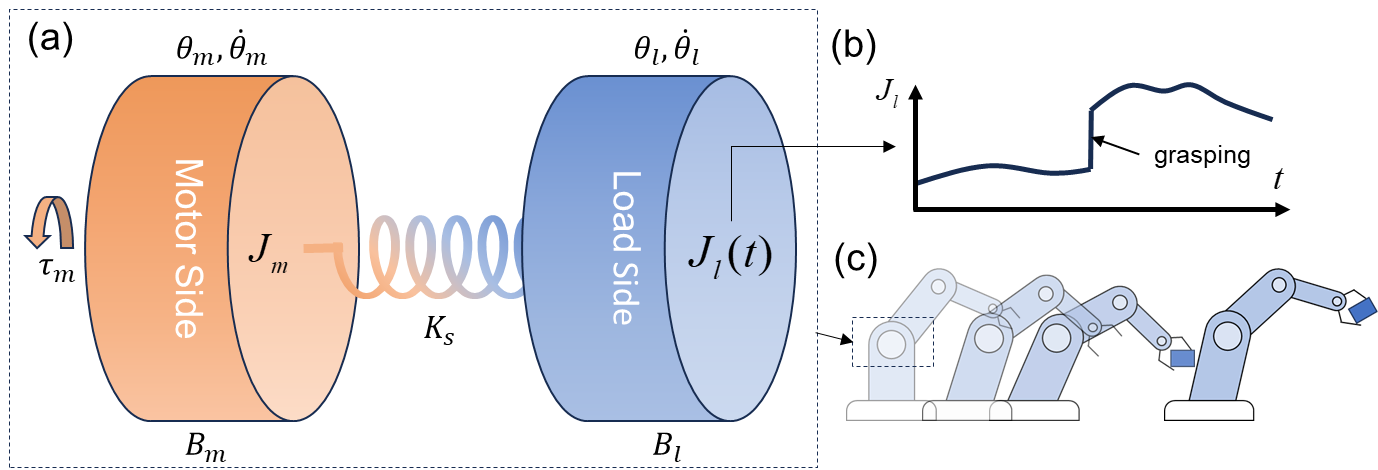
\includegraphics[width=0.48\textwidth]{figs/fig1png.png}
    \caption{Overview of the Series Elastic Actuator (SEA) control problem addressed in this work. \textbf{(a)} A rotational SEA is modeled as a motor side with inertia $J_m$ and a load side with time-varying inertia $J_l(t)$, mechanically coupled by a torsional spring of stiffness $K_s$. The motor applies torque $\tau_m$, while the motor-side and load-side angular positions, $\theta_m$ and $\theta_l$, are measured independently. Their difference, $\Delta\theta=\theta_m-\theta_l$, is the spring deflection and is directly related to the transmitted torque. \textbf{(b)} In a representative manipulation task, payload attachment and release produce abrupt step-like changes in $J_l(t)$ over a wide range. These inertia transients alter the coupled SEA dynamics and motivate the proposed TRACE framework.}
    \label{fig:sea_overview}
\end{figure}

Since the introduction of SEAs for safe physical human--robot interaction~\cite{pratt1995Series,pratt1999Series}, control design has largely focused on balancing mechanical compliance, closed-loop bandwidth, and force or position tracking accuracy~\cite{calanca2016Review,paine2014Design}. Classical cascaded position--force control and impedance-control methods~\cite{hogan1985Impedance} can achieve good performance when the plant remains close to its nominal model. The same compliance that improves interaction safety, however, creates a resonant two-inertia system whose poles vary with the payload. This sensitivity becomes more pronounced when SEA joints are embedded in flexible or multi-body systems such as anthropomorphic manipulators~\cite{li2024Advances}. Abrupt load changes can therefore shift the dominant dynamics and invalidate fixed controller parameters within a single task.

Model-based controllers, including Linear Quadratic Regulators (LQR)~\cite{sariyildiz2026Robust} and model predictive control (MPC)~\cite{zhang2024Development}, rely on an accurate model or a sufficiently representative linearization. Their structure and constraint-handling properties are attractive, but their tracking performance can degrade when the true inertia departs substantially from the design value. Robust and observer-based methods reduce this sensitivity by estimating lumped disturbances or compensating unmodeled dynamics. Disturbance-observer-based SEA controllers have been developed to improve disturbance rejection and output stiffness~\cite{asignacion2021high,ito2024disturbance}, with extensions including variable disturbance observers~\cite{sun2025Variablea} and nonlinear observers for multi-joint systems~\cite{han2021nonlinear}. Impedance, admittance, active-disturbance-rejection, and sliding-mode methods provide further robustness for uncertain interaction tasks~\cite{lee2021hybrid,ozdemir2025adaptive,zhong2021toward,chen2021practical,sun2021trajectory}.

Adaptive controllers explicitly estimate uncertain parameters or update control gains online. Adaptive observers and parameter-estimation schemes have been incorporated into SEA control loops~\cite{song2025adaptive,min2026adaptive}, while hybrid adaptive control~\cite{lanh2023Hybrid} and $\mathcal{L}_1$ adaptive resonance-ratio control~\cite{min2024L1adaptive} improve robustness to structured uncertainty. Abrupt inertia transients nevertheless remain difficult. Observer bandwidth cannot be increased indefinitely without amplifying measurement noise, parameter adaptation requires informative excitation, and aggressive gain updates can excite the elastic mode. As a result, a controller may be accurate in steady state yet still exhibit estimation lag, overshoot, or conservative action immediately after payload attachment or release.

Learning-based control offers another route by learning control policies and adaptation mechanisms from interaction data. PPO~\cite{schulman2017Proximal} and related deep reinforcement-learning methods have been applied to SEA force control and dynamic-performance improvement~\cite{sambhus2023real,lahmann2025series,xia2026high}. Neural dynamic models and learning-augmented MPC have also been investigated for nonlinear elastic-actuator behavior~\cite{umurzakov2025neural,zhang2024Development}, and learning-based whole-body controllers have enabled SEA-equipped mobile manipulators to execute complex tasks~\cite{liu2021whole,ren2022integrated}. Although these methods can represent nonlinear coupled dynamics, a monolithic policy may generalize poorly when hidden physical parameters change outside the conditions represented by the current observation.

History-conditioned teacher--student adaptation provides a practical mechanism for handling such hidden parameters. The Rapid Motor Adaptation (RMA) framework~\cite{kumar2021RMA}, for example, trains a teacher policy with privileged physical information and then learns a student encoder that reconstructs an adaptation latent from observation history. This paradigm is attractive for sim-to-real deployment because privileged quantities are required only during training. Conventional RMA-style architectures, however, usually compress all unobserved environment properties into a single latent representation. For SEA control, this representation must simultaneously capture abrupt load-inertia changes and more slowly varying or weakly observable effects such as friction, damping, and spring-stiffness mismatch. A single temporal encoder must therefore compromise between emphasizing recent samples for fast adaptation and aggregating a longer history for robust latent inference.

To address this limitation, we propose TRACE, short for \emph{Timescale-Resolved Adaptation via Cross-Attention and Temporal Encoding}. TRACE constructs a structured adaptation state rather than a single undifferentiated latent vector. A Fast Attention v2 Branch uses short- and long-horizon cross-attention to produce bounded load-inertia estimates, which are fused by a learned jump gate. In parallel, a Slow TCN Branch infers latent residual dynamics over the full history window. The estimated inertia and latent dynamics are supplied to a policy trained with privileged information, but deployment uses only measurable observation history. The term \emph{timescale-resolved} refers to this functional separation of rapidly changing and slowly inferred effects; both branches still execute in every 200~Hz control cycle.

\subsection{Contributions}

The main contributions of this work are summarized as follows:

\begin{enumerate}
    \item \textbf{Timescale-resolved adaptation architecture}: TRACE separates explicit load-inertia estimation from slower latent-dynamics inference through parallel attention and TCN branches.

    \item \textbf{Bounded dual-timescale inertia estimation}: The Fast Attention v2 Branch fuses short- and long-horizon estimates through a jump gate and is refined by closed-loop DAgger over diverse friction and trajectory conditions.

    \item \textbf{Control accuracy and deployment feasibility}: TRACE achieves 0.0140~rad RMSE in the matched transient simulation benchmark, and the final control-only ONNX graph satisfies the neural-inference portion of the 200~Hz deadline on Jetson Orin with two CPU threads.
\end{enumerate}

The remainder of this paper is organized as follows. Section~II formulates the control problem and presents the SEA dynamics. Section~III describes the TRACE architecture, including the privileged teacher policy, the timescale-resolved student branches, and the training procedure. Section~IV defines the matched simulation protocol and baselines. Section~V presents the main benchmark, adaptation diagnostics, cross-condition generalization, and deployment timing. Section~VI discusses the observed tradeoffs and evidence boundaries. Section~VII describes the physical SEA testbench and hardware-validation protocol. Section~VIII concludes the paper.

\section{Problem Formulation}

\subsection{SEA System Dynamics}

The fundamental physical challenge addressed in this work is illustrated in Fig. \ref{fig:sea_overview}. As shown in Fig. \ref{fig:sea_overview}(a), the SEA is conventionally modeled as a two-mass system consisting of a motor and a load, coupled by a compliant spring element. However, unlike traditional nominal models that assume constant physical properties, the load inertia $J_l(t)$ in our formulation is explicitly defined as a time-varying parameter to reflect practical dynamic manipulation tasks. The system dynamics can be described by the following coupled differential equations:

\begin{equation}
\begin{aligned}
J_m \ddot{\theta}_m &= \tau_m - K_s(\theta_m - \theta_l) - B_m\dot{\theta}_m - \tau_{f,m}, \\
J_l \ddot{\theta}_l &= K_s(\theta_m - \theta_l) - B_l\dot{\theta}_l - \tau_{f,l}.
\end{aligned}
\label{eq:sea_dynamics}
\end{equation}

\noindent where $\theta_m$ and $\theta_l$ are the motor and load angular positions (rad), $J_m$ and $J_l$ are the motor and load inertias (kg$\cdot$m$^2$), $\tau_m$ is the motor torque (N$\cdot$m), $K_s$ is the spring stiffness (N$\cdot$m/rad), $B_m$ and $B_l$ are viscous damping coefficients (N$\cdot$m$\cdot$s/rad), and $\tau_{f,m}$ and $\tau_{f,l}$ represent Coulomb friction torques (N$\cdot$m).
In this study, load-inertia variations are modeled as piecewise-constant payload changes caused by attachment, release, or clutch engagement events. Between two events, $J_l$ is constant and the standard two-inertia SEA dynamics in~\eqref{eq:sea_dynamics} are used. At the switching instant, the inertia change is treated as an external hybrid event applied between discrete control updates; impact dynamics and momentum exchange during the infinitesimal transition are not modeled explicitly. Therefore, the additional $\dot{J}_l\dot{\theta}_l$ term associated with continuously moving mass redistribution is outside the scope of the nominal model. This assumption matches the simulation benchmark and the planned clutch-based testbench, where the controller is evaluated on recovery after discrete inertia transitions rather than on the detailed contact mechanics of the switching event.

As depicted in Fig.~\ref{fig:sea_overview}, payload attachment or release produces a discrete change in the reflected load inertia. The resulting shift in resonant dynamics can invalidate fixed controller parameters before a conventional estimator has converged. This motivates a timescale-resolved architecture that reacts to abrupt inertia changes while retaining a longer context for residual dynamics.


\begin{figure*}[t]
\centering
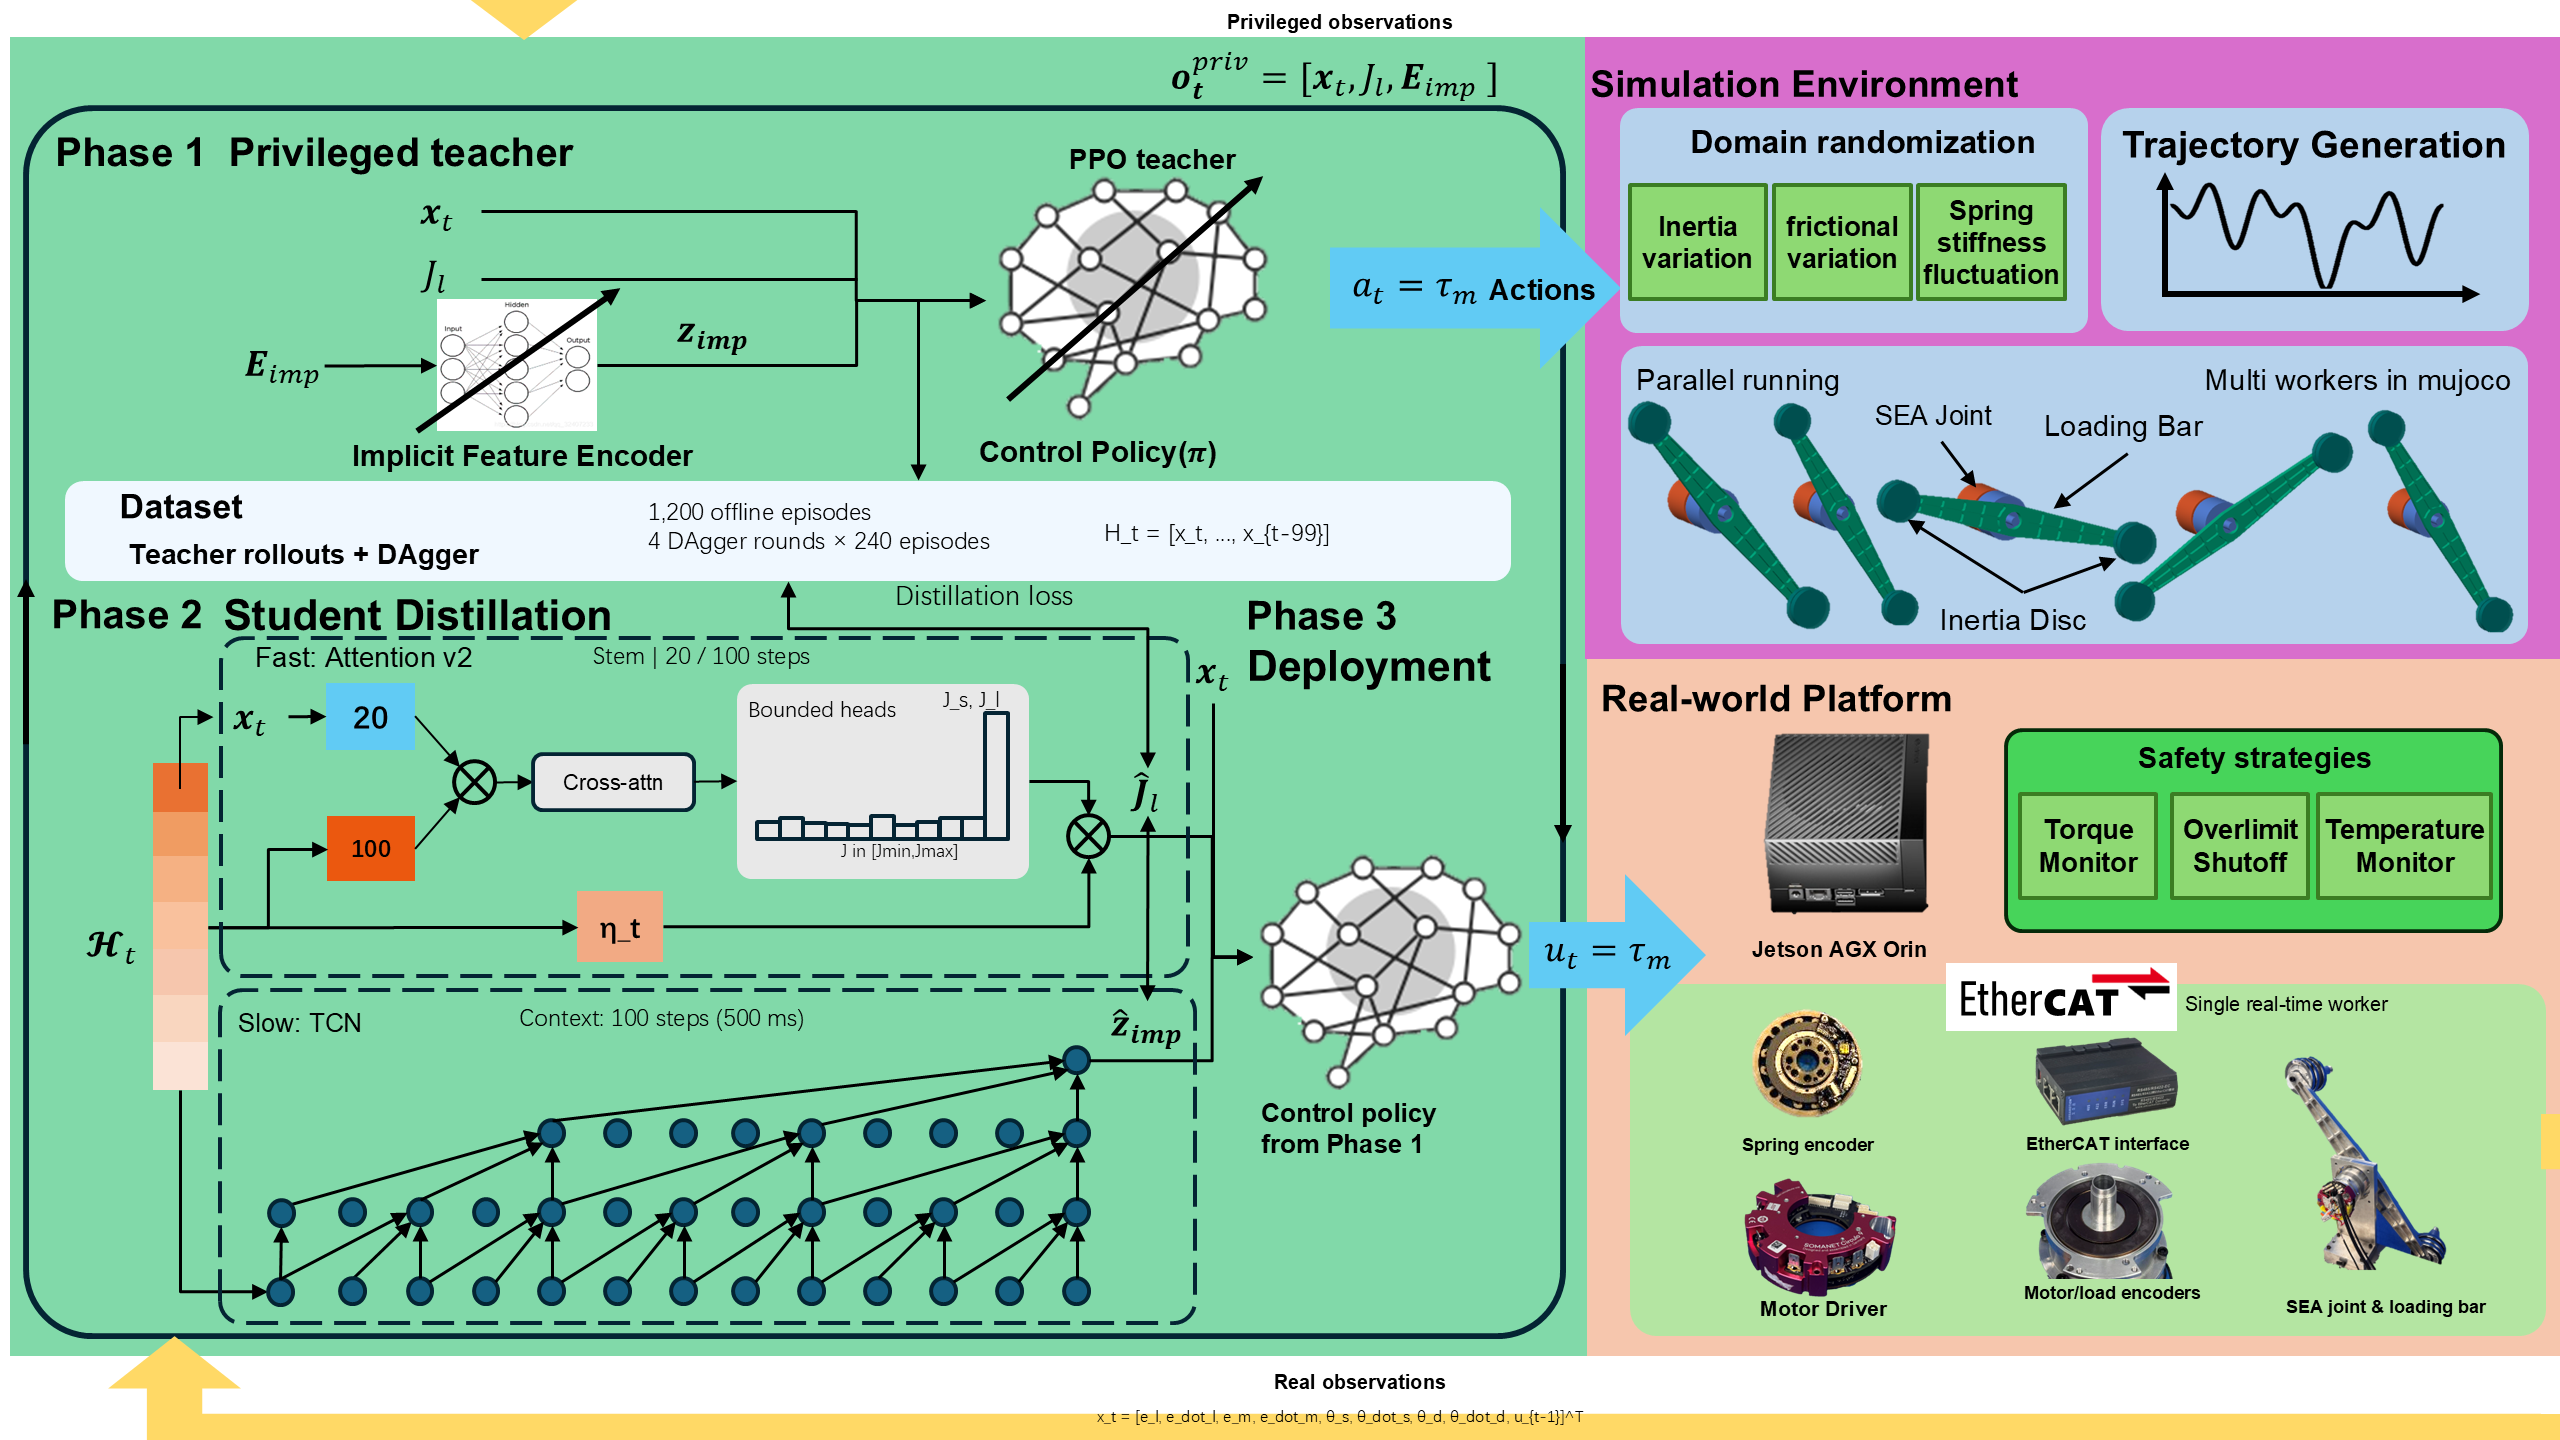
\includegraphics[width=0.96\textwidth]{figs/fig2png.png}
\caption{TRACE training and deployment pipeline. \textbf{Phase 1:} A PPO teacher is trained with privileged load inertia $J_l$ and encoded residual parameters. \textbf{Phase 2:} The frozen teacher supplies targets for a Fast Attention v2 Branch and a Slow TCN Branch. The fast branch fuses bounded short- and long-horizon inertia estimates, while the slow branch estimates latent residual dynamics from a 100-step history. \textbf{Phase 3:} The student branches and deterministic teacher actor run from non-privileged observation history $\mathcal{H}_t$ only.}
\label{fig:trace_architecture}
\end{figure*}


The spring deflection $\Delta\theta = \theta_m - \theta_l$ provides a measure of the transmitted torque:
\begin{equation}
\tau_s = K_s \Delta\theta \label{eq:spring_torque}
\end{equation}

\subsection{Time-Varying Inertia Challenge}

In practical applications, the load inertia $J_l(t)$ varies due to payload changes, human-robot interaction forces, or dynamic manipulation tasks. We consider the scenario where:
\begin{equation}
J_l(t) \in [J_{\min}, J_{\max}], \quad \frac{J_{\max}}{J_{\min}} \gg 1 \label{eq:inertia_range}
\end{equation}

In our experiments, $J_l(t) \in [0.05, 1.0]$ kg$\cdot$m$^2$, representing a 20-fold variation range. The controller has no prior knowledge of when the discrete inertia transitions occur or which value will follow each transition.

\subsection{Control Objective}

Given a desired trajectory $\theta_d(t)$ and its derivatives $\dot{\theta}_d(t)$, $\ddot{\theta}_d(t)$, the control objective is to design a feedback controller that computes motor torque $\tau_m(t)$ such that the load position $\theta_l(t)$ tracks the reference with minimal error:
\begin{equation}
\min_{\tau_m} \int_0^T \left[ w_p(\theta_l - \theta_d)^2 + w_v(\dot{\theta}_l - \dot{\theta}_d)^2 + w_u \tau_m^2 \right] dt \label{eq:objective}
\end{equation}

\noindent subject to torque constraints $|\tau_m| \leq \tau_{\max}$ and stability requirements.

\subsection{Observation Space}

The controller has access to the following 9-dimensional observation vector at each control timestep:
\begin{equation}
\bm{x}_t = \begin{bmatrix}
e_{l} & \dot{e}_{l} & e_{m} & \dot{e}_{m} & \theta_s & \dot{\theta}_s & \theta_d & \dot{\theta}_d & u_{t-1}
\end{bmatrix}^\mathrm{T} \label{eq:observation}
\end{equation}

\noindent where $e_{l} = \theta_d - \theta_l$ and $\dot{e}_{l} = \dot{\theta}_d - \dot{\theta}_l$ are load-side tracking errors, $e_{m} = \theta_d - \theta_m$ and $\dot{e}_{m} = \dot{\theta}_d - \dot{\theta}_m$ are motor-side tracking errors with respect to the same reference trajectory, $\theta_s$ and $\dot{\theta}_s$ are spring deflection and rate, $\theta_d$ and $\dot{\theta}_d$ are reference position and velocity, and $u_{t-1} \in [-1, 1]$ is the previous normalized control action.

Critically, the observation does not include the load inertia $J_l$ or friction parameters, which must be estimated from observation history.

\subsection{Key Challenges}

Controlling SEAs with time-varying inertia presents several fundamental challenges:

\begin{enumerate}
\item \textbf{History-Based Estimation}: During smooth tracking, acceleration can be small over part of a cycle, making inertia weakly observable from a single sample. TRACE therefore uses finite input--output history and relies on excitation from the commanded and closed-loop motion.

\item \textbf{Rapid Adaptation}: When inertia changes abruptly (e.g., payload release), the controller must adapt quickly enough to limit the resulting tracking transient.

\item \textbf{Multiple Temporal Contexts}: Abrupt inertia events emphasize recent samples, whereas friction, damping, and stiffness mismatch require a longer context for robust inference.

\item \textbf{Deployment Constraints}: Real-time control at 200 Hz requires end-to-end inference latency below the 5 ms control period and memory footprint suitable for embedded systems.
\end{enumerate}

TRACE addresses these challenges by separating explicit inertia estimation from longer-context latent-dynamics inference, as detailed in Section~III.

\section{TRACE Architecture}

TRACE consists of two training phases: a privileged teacher policy is first trained by reinforcement learning, after which two timescale-specialized student branches are trained to reconstruct its structured adaptation state from observation history. Fig.~\ref{fig:trace_architecture} summarizes the architecture and deployment path.

\subsection{Teacher Policy with Privileged Information}

\subsubsection{Privileged Observation Space}

During training, the teacher policy has access to privileged information that is unavailable during deployment:
\begin{equation}
\bm{o}_t^{\text{priv}} = \begin{bmatrix}
\bm{x}_t^\mathrm{T} & J_l & \bm{E}_{\text{imp}}^\mathrm{T}
\end{bmatrix}^\mathrm{T} \in \mathbb{R}^{15} \label{eq:priv_obs}
\end{equation}

\noindent where $\bm{x}_t \in \mathbb{R}^9$ is the base observation (Eq.~\ref{eq:observation}), $J_l \in \mathbb{R}$ is the ground-truth load inertia, and $\bm{E}_{\text{imp}} \in \mathbb{R}^5$ contains implicit parameters:
\begin{equation}
\bm{E}_{\text{imp}} = \begin{bmatrix}
\tau_{c,m} & \tau_{c,l} & B_m & B_l & \Delta K_s
\end{bmatrix}^\mathrm{T} \label{eq:implicit_params}
\end{equation}

\noindent representing motor and load Coulomb friction ($\tau_{c,m}$, $\tau_{c,l}$), viscous damping coefficients ($B_m$, $B_l$), and spring stiffness deviation ($\Delta K_s$).

\subsubsection{Implicit Feature Encoder}

To reduce dimensionality and extract relevant features from $\bm{E}_{\text{imp}}$, we employ a two-layer MLP encoder:
\begin{equation}
\begin{aligned}
\bm{h}_1 &= \text{ELU}(\bm{W}_1 \bm{E}_{\text{imp}} + \bm{b}_1), \quad \bm{W}_1 \in \mathbb{R}^{16 \times 5}, \\
\bm{z}_{\text{imp}} &= \bm{W}_2 \bm{h}_1 + \bm{b}_2, \quad \bm{W}_2 \in \mathbb{R}^{8 \times 16}.
\end{aligned}
\label{eq:encoder_z}
\end{equation}

\noindent where $\bm{z}_{\text{imp}} \in \mathbb{R}^8$ is the implicit feature vector. The teacher policy then operates on the 18-dimensional feature vector:
\begin{equation}
\bm{f}_t = \begin{bmatrix}
\bm{x}_t^\mathrm{T} & J_l & \bm{z}_{\text{imp}}^\mathrm{T}
\end{bmatrix}^\mathrm{T} \in \mathbb{R}^{18} \label{eq:teacher_features}
\end{equation}

\subsubsection{Policy Network}

The teacher policy is parameterized as a Gaussian policy:
\begin{equation}
\begin{aligned}
\bm{\mu}_t &= \pi_\theta(\bm{f}_t) = \text{MLP}(\bm{f}_t) \in \mathbb{R}, \\
u_t &\sim \mathcal{N}(\mu_t, \sigma^2).
\end{aligned}
\label{eq:teacher_policy}
\end{equation}

\noindent where the MLP consists of two hidden layers with 128 units each and ELU activations. The log standard deviation $\log \sigma$ is a learnable parameter initialized to $-0.5$.

\subsubsection{Training Objective}

The teacher policy is trained using Proximal Policy Optimization (PPO)~\cite{schulman2017Proximal} to maximize the expected return:
\begin{equation}
\mathcal{J}(\theta) = \mathbb{E}_{\tau \sim \pi_\theta} \left[ \sum_{t=0}^T \gamma^t r_t \right] \label{eq:ppo_objective}
\end{equation}

The base reward encourages accurate tracking while penalizing excessive control effort and abrupt action changes:
\begin{align}
r_t = &\, r_{\text{alive}} + r_{\text{precision}} - w_p e_{l}^2 - w_v \dot{e}_{l}^2 \nonumber \\
&- w_s \theta_s^2 - w_u \tau_m^2 - w_{\Delta u} (\Delta \tau_m)^2. \label{eq:reward}
\end{align}

\noindent Here, $r_{\text{alive}}=1.0$ and $r_{\text{precision}}=5.0\exp[-e_l^2/(0.05)^2]$. The base weights are $w_p=1.5$, $w_v=0.02$, $w_s=1.0$, $w_u=0.001$, and $w_{\Delta u}=0.005$. During the first 0.3~s after a sampled inertia jump, an additional linearly decaying penalty emphasizes position error, velocity error, spring deflection and velocity, effort, action increments, and spring-torque increments. Its weights are 4.0, 0.04, 1.0, 0.03, 0.0002, 0.004, and 0.0015, respectively; downward jumps receive a factor of 1.8. This event term is used only during teacher refinement and does not require event timing at deployment.

The final reported teacher is initialized from a composite-trajectory policy and refined for 4 million timesteps in 16 parallel environments, with domain randomization over inertia ($J_l \in [0.05, 1.0]$ kg$\cdot$m$^2$), friction parameters, and trajectory characteristics. Inertia-jump episodes are oversampled during this refinement.

\subsection{Fast Attention v2 Branch for Inertia Estimation}

The Fast Attention v2 Branch estimates load inertia $\hat{J}_l$ from observation history. Its deployment inputs are limited to measurable SEA signals: motor and load velocities, finite-difference accelerations, spring deflection and velocity, spring torque computed from nominal stiffness, and the previous action. It does not use friction coefficients, viscous damping, oracle inertia, or oracle latent features. The estimator exploits excitation in the tested trajectories but does not claim inertia identifiability under arbitrary zero-excitation motion.

\subsubsection{History Window Construction}

At each timestep $t$, we maintain a FIFO queue of the most recent $L = 100$ observations:
\begin{equation}
\mathcal{H}_t = \{\bm{x}_{t-L+1}, \bm{x}_{t-L+2}, \ldots, \bm{x}_t\} \in \mathbb{R}^{L \times 9} \label{eq:history_window}
\end{equation}

The window length $L = 100$ corresponds to 0.5 seconds at 200 Hz control frequency, providing sufficient temporal context for inertia estimation while maintaining computational efficiency.

\subsubsection{Dual-Timescale Current-to-History Attention}

The v2 estimator maps each observation history to an 8-dimensional measurable dynamics feature vector:
\begin{equation}
\begin{aligned}
\bm{\phi}_i = [&\dot{\theta}_{l,i}, \ddot{\theta}_{l,i}, \dot{\theta}_{m,i}, \ddot{\theta}_{m,i}, \\
&\theta_{s,i}, \dot{\theta}_{s,i}, \tau_{s,i}, u_{i-1}]^\mathrm{T}.
\end{aligned}
\label{eq:fast_features}
\end{equation}

\noindent Fixed physical scales normalize these features before a temporal convolutional stem produces encoded tokens $\bm{e}_{t-L+1:t}\in\mathbb{R}^{L\times d}$. The newest token queries short and long attention paths:
\begin{equation}
\begin{aligned}
\bm{c}_{s,t} &= \mathrm{MHA}_s(\bm{e}_t,\bm{e}_{t-L_s+1:t},\bm{e}_{t-L_s+1:t}), \\
\bm{c}_{\ell,t} &= \mathrm{MHA}_{\ell}(\bm{e}_t,\bm{e}_{t-L+1:t},\bm{e}_{t-L+1:t}),
\end{aligned}
\label{eq:dual_attention}
\end{equation}

\noindent where $L=100$, $L_s=20$, and $d=128$; each path uses eight heads. The short path emphasizes recent transients, while the long path preserves broader context. Their outputs are mapped to bounded estimates and fused by a learned jump gate:
\begin{equation}
\begin{aligned}
\hat{J}_{s,t} &= J_{\min}+(J_{\max}-J_{\min})\sigma(g_s(\bm{c}_{s,t},\bm{e}_t)), \\
\hat{J}_{\ell,t} &= J_{\min}+(J_{\max}-J_{\min})\sigma(g_{\ell}(\bm{c}_{\ell,t},\bm{e}_t)), \\
\eta_t &= \sigma(g_{\eta}(\bm{c}_{s,t},\bm{c}_{\ell,t},\bm{e}_t)), \\
\hat{J}_t &= \eta_t\hat{J}_{s,t}+(1-\eta_t)\hat{J}_{\ell,t}.
\end{aligned}
\label{eq:inertia_estimate}
\end{equation}

\subsubsection{Timescale-Resolved Fusion}

The gate $\eta_t$ is supervised to favor the short path near inertia jumps and the long path during steady segments. This learned fusion is evaluated every control cycle and therefore requires no external change detector. The gate head also returns confidence for diagnostics, but deployment uses the raw bounded estimate in~\eqref{eq:inertia_estimate}. A fixed confidence hold is avoided because it can preserve an outdated inertia estimate during weak excitation.

The Fast Attention v2 Branch is trained with regression, branch-specific, jump-gate, and confidence terms:
\begin{equation}
\mathcal{L}_{\text{fast}}=\mathcal{L}_{\text{reg}}+\lambda_r\mathcal{L}_{\text{rel}}+\lambda_s\mathcal{L}_s+\lambda_{\ell}\mathcal{L}_{\ell}+\lambda_g\mathcal{L}_g+\lambda_c\mathcal{L}_c.
\label{eq:fast_loss}
\end{equation}

\noindent The regression terms supervise the fused, short, and long estimates. The auxiliary terms train transition-sensitive gating and confidence without introducing privileged deployment inputs.

\subsection{Slow TCN Branch for Implicit Feature Extraction}

While the Fast Attention v2 Branch estimates explicit inertia, the Slow TCN Branch extracts implicit friction, damping, and stiffness features over a longer temporal context.

\subsubsection{Causal Temporal Convolutional Network}

We employ a five-layer causal dilated convolutional network that processes the same history window $\mathcal{H}_t$. The input is first permuted to channel-first format $(B, 9, L)$ for 1D convolution.

Each layer consists of a causal convolution with dilation, layer normalization, and ELU activation:
\begin{equation}
\begin{aligned}
\bm{h}_1 &= \text{ELU}(\text{LN}(\text{Conv1D}_{d=1}^{k=8}(\mathcal{H}_t))) \in \mathbb{R}^{64 \times L}, \\
\bm{h}_2 &= \text{ELU}(\text{LN}(\text{Conv1D}_{d=2}^{k=8}(\bm{h}_1))) \in \mathbb{R}^{128 \times L}, \\
\bm{h}_3 &= \text{ELU}(\text{LN}(\text{Conv1D}_{d=4}^{k=8}(\bm{h}_2))) \in \mathbb{R}^{128 \times L}, \\
\bm{h}_4 &= \text{ELU}(\text{LN}(\text{Conv1D}_{d=8}^{k=4}(\bm{h}_3))) \in \mathbb{R}^{64 \times L}, \\
\bm{h}_5 &= \text{ELU}(\text{LN}(\text{Conv1D}_{d=16}^{k=4}(\bm{h}_4))) \in \mathbb{R}^{32 \times L}.
\end{aligned}
\label{eq:tcn_stack}
\end{equation}

\noindent where $k$ denotes kernel size and $d$ denotes dilation rate. Causal padding ensures that the output at time $t$ depends only on inputs up to time $t$, maintaining causality for real-time deployment.

The effective receptive field grows exponentially with dilation:
\begin{equation}
\text{RF} = 1 + \sum_{l=1}^5 d_l (k_l - 1) = 122 \text{ steps} \label{eq:receptive_field}
\end{equation}

Since the FIFO window contains 100 real observations, the effective real-data context is the full 100-step history, corresponding to 500 ms at 200 Hz. This horizon provides longer context for latent residual-dynamics inference while remaining computationally efficient.

\subsubsection{Output Projection}

The final temporal feature at time $t$ is extracted and projected to the 8-dimensional implicit feature space:
\begin{equation}
\hat{\bm{z}}_{\text{imp}} = \bm{W}_{\text{out}} \bm{h}_5[:, -1] + \bm{b}_{\text{out}} \in \mathbb{R}^8 \label{eq:slow_output}
\end{equation}

\noindent where $\bm{h}_5[:, -1]$ selects the feature vector corresponding to the most recent timestep.

\subsubsection{Slow-Branch Distillation Loss}

The frozen Slow checkpoint was trained with target MSE and a weak minibatch-consistency term:
\begin{equation}
\mathcal{L}_{\text{slow}} = \mathbb{E} \left[ \|\hat{\bm{z}}_{\text{imp}} - \bm{z}_{\text{imp}}\|^2 + \lambda \|\hat{\bm{z}}_{\text{imp}}^{(i)} - \hat{\bm{z}}_{\text{imp}}^{(i-1)}\|^2 \right], \label{eq:slow_loss}
\end{equation}

\noindent where $i$ indexes adjacent entries in a shuffled training minibatch and $\lambda=0.05$. Accordingly, this legacy term is a weak output-contraction regularizer, not a temporal-derivative penalty. The temporal behavior of the Slow branch is therefore evaluated from causal closed-loop rollouts rather than inferred from this term. A sequence-aware replacement is identified as future implementation work.

\subsection{Student Network Training}

\subsubsection{Data Collection}

After training the teacher policy to convergence, we freeze its parameters and collect a dataset by rolling out the teacher in diverse environments. For each episode, we record:
\begin{itemize}
\item History windows: $\mathcal{H}_t \in \mathbb{R}^{100 \times 9}$
\item Ground-truth inertia: $J_l \in \mathbb{R}$
\item Teacher's implicit features: $\bm{z}_{\text{imp}} \in \mathbb{R}^8$ (from Eq.~\ref{eq:encoder_z})
\end{itemize}

For the Fast Attention v2 Branch, we collect 1,200 teacher-rollout episodes and retain 120 independent episodes for validation. The offline model is then refined through four DAgger rounds with teacher blend factors $\beta=0.8$, $0.5$, $0.2$, and $0.0$. Each round contributes 240 closed-loop rollout episodes and progressively exposes the estimator to the state distribution induced by the student controller.

\subsubsection{Supervised Distillation}

The Fast and Slow branches are trained by supervised distillation and integrated with the frozen teacher actor. Their total objective is
\begin{equation}
\mathcal{L}_{\text{total}} = \mathcal{L}_{\text{fast}} + \mathcal{L}_{\text{slow}} \label{eq:total_loss}
\end{equation}

Fast-branch checkpoints are selected by closed-loop evaluation rather than offline validation loss alone. The selection suite contains 108 independent conditions formed by six trajectory and inertia patterns, six load Coulomb-friction levels, and three load viscous-damping levels. The deployed estimator uses the raw bounded output; confidence is logged for diagnostics but does not trigger a hard hold.

\subsection{Deployment Pipeline}

During deployment, the complete inference pipeline is designed for the 200 Hz control loop:
\begin{enumerate}
\item Read 9D observation $\bm{x}_t$ from sensors
\item Update FIFO history buffer $\mathcal{H}_t$
\item Fast Attention v2 Branch: $\mathcal{H}_t \rightarrow \hat{J}_l$ (parallel)
\item Slow Branch: $\mathcal{H}_t \rightarrow \hat{\bm{z}}_{\text{imp}}$ (parallel)
\item Construct augmented observation: $\bm{f}_t = [\bm{x}_t^\mathrm{T}, \hat{J}_l, \hat{\bm{z}}_{\text{imp}}^\mathrm{T}]^\mathrm{T}$
\item Apply observation normalization (running mean/std from training)
\item Teacher policy: $\bm{f}_t \rightarrow u_t$
\item Denormalize and apply motor torque: $\tau_m = u_t \cdot \tau_{\max}$
\end{enumerate}

The Fast and Slow branches execute in parallel within each control cycle. Section~\ref{sec:computational_performance} reports the measured timing of the lightweight ONNX deployment path.

% Revised simulation evidence is modularized for figure and protocol iteration.
\section{Simulation Setup and Evaluation Protocol}
\label{sec:simulation_setup}

\subsection{SEA Model and Timing}

TRACE is evaluated in MuJoCo using the rotational SEA model in Fig.~\ref{fig:sea_overview}. The payload body translates along a radial slider, giving the effective inertia $J_l=J_{l,\mathrm{base}}+J_{l,\mathrm{payload}}+m_pr^2$ without directly modifying the MuJoCo inertia tensor during integration. Table~\ref{tab:system_params} lists the structural parameters used in all reported simulations.

\begin{table}[t]
\centering
\caption{SEA Simulation Parameters}
\label{tab:system_params}
\begin{tabular}{@{}lcc@{}}
\toprule
Parameter & Symbol & Value \\
\midrule
Motor inertia & $J_m$ & 0.417 kg$\cdot$m$^2$ \\
Base load inertia & $J_{l,\mathrm{base}}$ & 0.04 kg$\cdot$m$^2$ \\
Payload intrinsic inertia & $J_{l,\mathrm{payload}}$ & 0.01 kg$\cdot$m$^2$ \\
Evaluated load-inertia range & $J_l$ & 0.05--1.00 kg$\cdot$m$^2$ \\
Spring stiffness & $K_s$ & 3800 N$\cdot$m/rad \\
Passive motor-joint damping & $B_{m,0}$ & 0.0955 N$\cdot$m$\cdot$s/rad \\
Motor-torque limit & $\tau_{\max}$ & 61 N$\cdot$m \\
Control / simulation rate & $f_c/f_{\mathrm{sim}}$ & 200 / 1000 Hz \\
\bottomrule
\end{tabular}
\end{table}

The main benchmark fixes the additional friction and damping terms at $F_{c,m}=6.0$~N$\cdot$m, $F_{c,l}=0.2$~N$\cdot$m, $B_m=8.0$~N$\cdot$m$\cdot$s/rad, $B_l=0.01$~N$\cdot$m$\cdot$s/rad, and $\Delta K_s=0$. An inertia switch is applied between control updates without artificially rescaling the joint velocity. This isolates controller recovery from an imposed momentum-reset artifact.

\subsection{Training and Model Selection}

The privileged teacher was initialized from the composite-trajectory policy and refined for $4\times10^6$ steps in 16 parallel environments using inertia-jump-focused episodes. The student dataset contains 1200 offline teacher episodes and four 240-episode DAgger rounds; an independent 120-episode set is reserved for validation. The final Fast Attention v2 checkpoint is selected by closed-loop evaluation rather than by offline validation loss alone.

The PPO baseline uses the same 9-D instantaneous observation as TRACE but no history encoder. The RMA baseline~\cite{kumar2021RMA} uses one TCN to infer an 8-D latent vector and does not receive $J_l$ directly at deployment. To avoid reward-induced bias, the final RMA teacher is trained for $8\times10^6$ steps with the same base reward weights used by TRACE, followed by policy-aware student distillation from 3000 episodes. All learned controllers are frozen before the test trajectories are generated.

The tuned PD+DOB baseline uses $K_p=500$, $K_d=15$, $J_{\mathrm{nom}}=0.5$~kg$\cdot$m$^2$, a 20-Hz first-order disturbance filter, and a disturbance-compensation gain of 0.2. Increasing $K_d$ from 2 to 15 suppresses the periodic torque oscillation without changing the observer structure. The augmented LQR is designed at $J_{\mathrm{nom}}=0.3$~kg$\cdot$m$^2$ and yields the implemented feedback gain $\bm{K}_{\mathrm{LQR}}=[15.636,\,2.915,\,112.761,\,4.052]$ for $[e_l,\dot e_l,e_m,\dot e_m]^\mathrm{T}$.

\subsection{Evaluation Matrix and Metrics}

The decisive benchmark uses the fixed reference $q_d(t)=0.5\sin(2\pi\,0.3t)$~rad with zero phase, so the initial position error is zero. The load inertia is 0.3~kg$\cdot$m$^2$ initially, drops to 0.05~kg$\cdot$m$^2$ at $t=3$~s (payload release), and rises to 0.75~kg$\cdot$m$^2$ at $t=7$~s (payload attachment). Every controller receives the same reference, physical parameters, switch times, and random seed.

We report full-episode tracking RMSE, 0.5-s post-event RMSE, RMS motor torque, RMS torque increment $\mathrm{RMS}(\Delta\tau_m)$, saturation rate, and inertia-estimation RMSE where applicable. Generalization is evaluated over 108 deterministic closed-loop conditions: six trajectory/inertia families, $F_{c,l}\in\{0,0.1,\ldots,0.5\}$~N$\cdot$m, and $B_l\in\{0,0.01,0.03\}$~N$\cdot$m$\cdot$s/rad. Because each condition uses one seed, this suite measures coverage and worst-case behavior rather than sampling uncertainty.

\section{Simulation Results}

\subsection{Abrupt-Inertia Tracking Benchmark}

To test whether explicit fast adaptation improves closed-loop behavior, all five controllers were evaluated under the same $0.3\rightarrow0.05\rightarrow0.75$~kg$\cdot$m$^2$ sequence. Fig.~\ref{fig:sim_main} aligns the position, error, torque, and TRACE inertia estimate on a shared time axis and enlarges the two post-switch evaluation windows.

\begin{figure*}[t]
\centering
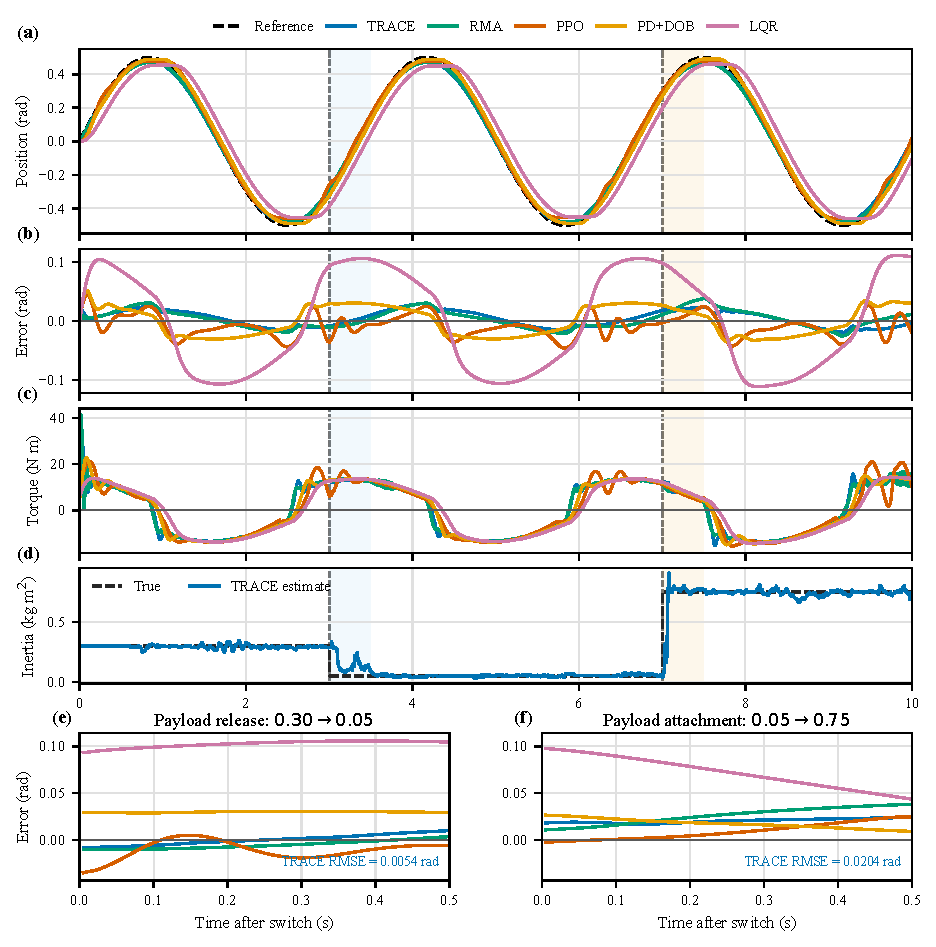
\includegraphics[width=0.96\textwidth]{fig_sim_main_comparison.pdf}
\caption{Closed-loop comparison under abrupt load-inertia changes. \textbf{(a)} Reference and load position. \textbf{(b)} Tracking error. \textbf{(c)} Applied motor torque. \textbf{(d)} True and TRACE-estimated load inertia. \textbf{(e,f)} Tracking-error responses in the shaded 0.5-s windows after payload release and attachment. The reference has zero phase and hence zero initial position error; vertical dashed lines mark the two events.}
\label{fig:sim_main}
\end{figure*}

\begin{table}[t]
\centering
\caption{Abrupt-Inertia Benchmark; Lower Is Better}
\label{tab:main_benchmark}
\footnotesize
\begin{tabular}{@{}lcccc@{}}
\toprule
Method & Overall & Release & Attach. & $\mathrm{RMS}(\Delta\tau)$ \\
& RMSE & RMSE & RMSE & (N$\cdot$m) \\
\midrule
TRACE & \textbf{0.0140} & \textbf{0.0054} & 0.0204 & 0.4156 \\
RMA & 0.0154 & 0.0068 & 0.0274 & 1.0879 \\
PPO & 0.0203 & 0.0145 & \textbf{0.0125} & 0.2797 \\
PD+DOB & 0.0248 & 0.0298 & 0.0181 & 0.2123 \\
LQR & 0.0821 & 0.1026 & 0.0739 & \textbf{0.1273} \\
\bottomrule
\end{tabular}
\end{table}

TRACE achieved the lowest full-episode RMSE, reducing it by 9.1\% relative to the same-reward RMA baseline, 31.1\% relative to PPO, 43.6\% relative to PD+DOB, and 83.0\% relative to LQR. It also produced the smallest error in the 0.5-s window after payload release. PPO had the lowest immediate post-attachment RMSE, showing that TRACE did not dominate every local transient, but PPO accumulated more error over the complete trajectory. None of the controllers saturated in this zero-phase test. TRACE was smoother than RMA but had larger torque increments than PPO, PD+DOB, and LQR, which exposes a tracking--smoothness tradeoff rather than an unconditional advantage.

\subsection{Timescale-Resolved Adaptation Dynamics}

Figs.~\ref{fig:sim_adaptation} and~\ref{fig:sim_attention} examine the Fast Attention v2 Branch around the two events. The short and long estimates remain close in steady regimes but respond differently while the 100-sample history is being replaced. The learned gate blends these estimates, while the event windows show how attention redistributes over recent and older samples.

\begin{figure}[t]
\centering
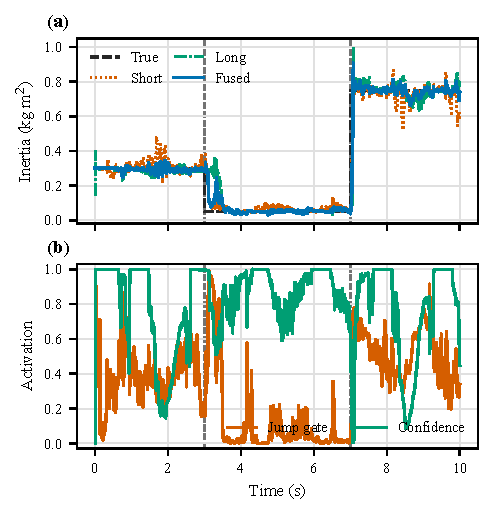
\includegraphics[width=\columnwidth]{fig_sim_adaptation_estimates.pdf}
\caption{Fast-branch adaptation outputs. \textbf{(a)} True inertia, short- and long-head estimates, and learned fusion. \textbf{(b)} Jump gate and confidence.}
\label{fig:sim_adaptation}
\end{figure}

\begin{figure}[t]
\centering
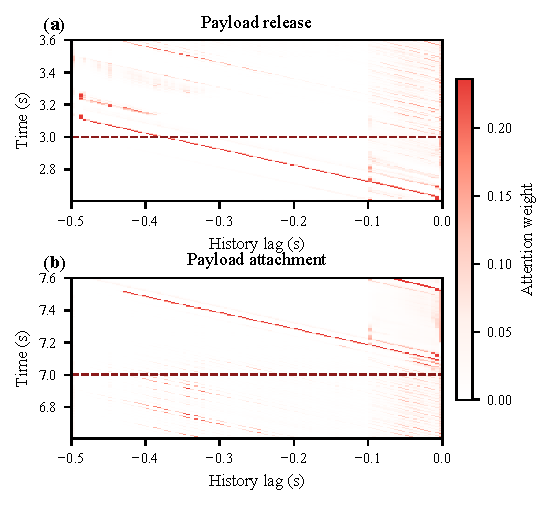
\includegraphics[width=\columnwidth]{fig_sim_attention_windows.pdf}
\caption{Attention weights around \textbf{(a)} payload release and \textbf{(b)} payload attachment. Zero lag denotes the newest sample. The maps diagnose temporal routing rather than constitute a formal change detector.}
\label{fig:sim_attention}
\end{figure}

In the zero-phase main benchmark, the fused estimate obtained stable-segment RMSEs of 0.0165, 0.0081, and 0.0234~kg$\cdot$m$^2$ in the three inertia regimes. The upward $0.05\rightarrow0.75$ transition produced the largest estimation excursion and coincided with TRACE's larger post-attachment tracking error. These diagnostics do not establish parameter identifiability.

\subsection{Cross-Condition Generalization and Failure Modes}

The 108-condition suite tests whether the fast estimator remains useful beyond the headline sinusoid. Figs.~\ref{fig:sim_generalization_inertia} and~\ref{fig:sim_generalization_tracking} report estimation and closed-loop tracking outcomes across trajectory, friction, and damping combinations.

\begin{figure}[t]
\centering
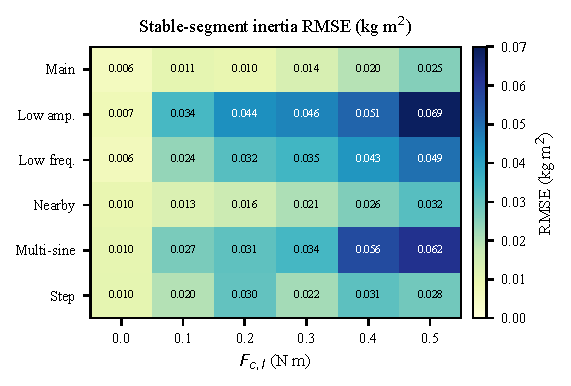
\includegraphics[width=\columnwidth]{fig_sim_generalization_inertia.pdf}
\caption{Stable-segment inertia RMSE over 108 conditions. Each cell averages three load-damping values.}
\label{fig:sim_generalization_inertia}
\end{figure}

\begin{figure}[t]
\centering
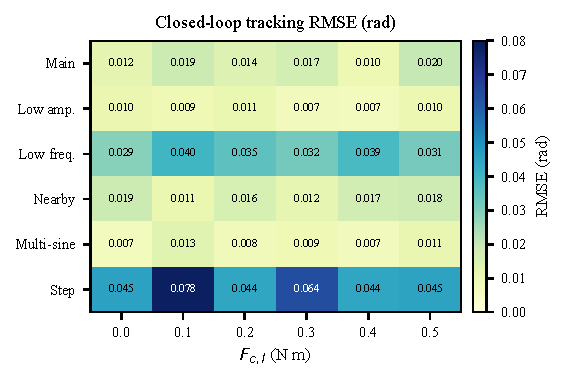
\includegraphics[width=\columnwidth]{fig_sim_generalization_tracking.pdf}
\caption{Closed-loop tracking RMSE for the same 108-condition suite.}
\label{fig:sim_generalization_tracking}
\end{figure}

Across all conditions, the final estimator achieved mean and worst stable-segment inertia RMSEs of 0.0279 and 0.0790~kg$\cdot$m$^2$, respectively. Estimation error generally increased with load Coulomb friction in low-amplitude and multi-sine cases, whereas step references produced the largest tracking errors even when inertia error was moderate. The contrasting heatmaps therefore show that accurate inertia estimation is helpful but not sufficient: reference smoothness, the Slow TCN latent, and the frozen policy also shape closed-loop error.

DAgger and output selection were also evaluated over this suite. The pre-DAgger confidence-hold model obtained mean/worst RMSEs of 0.0434/0.3771~kg$\cdot$m$^2$; after DAgger these became 0.0348/0.2495 with holding and 0.0279/0.0790 with the raw bounded output. Hard holding can preserve an outdated value during weak excitation, so the deployed controller records confidence only as a diagnostic.

\subsection{Deployment Latency}
\label{sec:computational_performance}

The final control-only ONNX graph contains Fast Attention v2, the Slow TCN, fixed observation normalization, and the deterministic actor. Table~\ref{tab:deployment_latency} separates workstation timing from measurements on the target Jetson Orin.

\begin{table}[t]
\centering
\caption{Final TRACE ONNX Latency at a 5-ms Deadline}
\label{tab:deployment_latency}
\footnotesize
\begin{tabular}{@{}lcccc@{}}
\toprule
Platform & Threads & Mean & P99 & Misses \\
& & (ms) & (ms) & \\
\midrule
Workstation CPU & 1 & 0.862 & 1.127 & 0/5000 \\
Jetson Orin CPU & 1 & 4.718 & 5.045 & 48/3000 \\
Jetson Orin CPU & 2 & 3.421 & 3.669 & 0/3000 \\
Jetson Orin CPU & 4 & 2.581 & 2.793 & 0/3000 \\
\bottomrule
\end{tabular}
\end{table}

The single-thread Orin run met the deadline on average but missed 1.6\% of cycles. Two CPU threads eliminated deadline misses in the measured run and left 1.33~ms of P99 margin; four threads increased that margin further. PyTorch--ONNX parity was verified with maximum absolute action error below $1.5\times10^{-6}$. These timings cover neural inference only and exclude sensing, EtherCAT communication, logging, and safety supervision.

\section{Discussion}

\subsection{Central Finding and Interpretation}

The matched zero-phase benchmark shows that TRACE improves full-episode tracking under the tested abrupt inertia sequence while preserving bounded torque and zero saturation. The advantage over the same-reward RMA baseline is 9.1\%, substantially smaller than in earlier unmatched comparisons but more defensible because both methods use deployment-only history and comparable reward shaping. Together with the stable inertia estimates in Fig.~\ref{fig:sim_main}(d), this result is consistent with explicit inertia information complementing a general latent adaptation vector.

This comparison does not establish that explicit inertia estimation is always superior. PPO achieved the lowest RMSE during the first 0.5~s after payload attachment, and the two 108-condition heatmaps show that low inertia RMSE does not necessarily imply low tracking RMSE. The frozen policy and Slow TCN latent can compensate for moderate estimation error, while a physically accurate estimate can still yield suboptimal tracking if the policy was not trained for the local reference dynamics.

\subsection{Transition Asymmetry and Control Smoothness}

The payload-release event was easier for TRACE than the 15-fold payload-attachment event. Both the fused estimate and tracking error showed a larger excursion after the upward transition. This asymmetry may reflect the larger dynamical change, the finite 0.5-s history replacement time, and reduced coverage of equally extreme upward transitions in closed-loop training. The mechanism plot supports temporal redistribution at both events, but it should not be interpreted as a formal detection guarantee.

TRACE also did not minimize every control-effort metric. Its torque-increment RMS was lower than RMA's but higher than those of PPO, tuned PD+DOB, and LQR. The classical controllers achieved smoother torque by accepting larger tracking error, whereas RMA combined relatively accurate tracking with the largest torque variation. Hardware evaluation should therefore report tracking and torque smoothness jointly rather than rank controllers by RMSE alone.

\subsection{Evidence Boundaries and Ablation Requirements}

RMA and PPO are algorithmic baselines, not strict component ablations: their policies, latent representations, and training procedures differ from TRACE. A submission-level component study should retrain or consistently evaluate full TRACE, a fixed-nominal-inertia variant, a Fast-only variant, short-only and long-only heads, fixed fusion, and the pre-DAgger estimator. This experiment is required to isolate the Slow TCN, dual-timescale heads, learned gate, and DAgger refinement independently.

The generalization suite contains broad deterministic coverage but only one seed per condition. Its distributions therefore describe condition-wise behavior rather than statistical confidence. Low-amplitude and multi-sine cases at high Coulomb friction produced the largest inertia errors, and step references produced the largest tracking errors. These cases identify weak excitation and reference discontinuity as current boundaries. Additional tests should vary sensor noise, encoder quantization, action delay, clutch timing, and unmodeled compliance before making a broad sim-to-real robustness claim.

\subsection{Deployment Implications}

The final ONNX graph fits within the 5-ms control period on the target Orin when at least two CPU inference threads are used. Single-thread mean latency alone is not sufficient: its 1.6\% deadline-miss rate would be unacceptable for deterministic control without scheduling safeguards. The remaining timing budget must also accommodate sensing, communication, safety checks, and logging. Consequently, the hardware implementation is configured for multi-thread inference, and validation must measure end-to-end cycle time rather than neural inference in isolation.

\section{Experimental Testbench}
\label{sec:testbench}

\subsection{Hardware Platform Overview}

To prepare for physical validation, we construct a single-DOF rotational SEA testbench with an electromagnetic-clutch-based variable-inertia load. The joint side carries an internal base inertia of 0.05 kg$\cdot$m$^2$. An external inertia module, consisting of a detachable long rod and end-mounted weights, can be coupled to or decoupled from the joint through a 24 V DLY0-10A electromagnetic clutch. When the clutch is engaged, the joint drives both the internal base inertia and the external rod-weight module. When the clutch is disengaged, only the internal base inertia remains connected to the SEA joint. This design physically realizes the abrupt inertia changes considered in the simulation study while allowing the next engaged inertia to be adjusted during the disengaged interval.

\begin{figure}[!t]
\centering
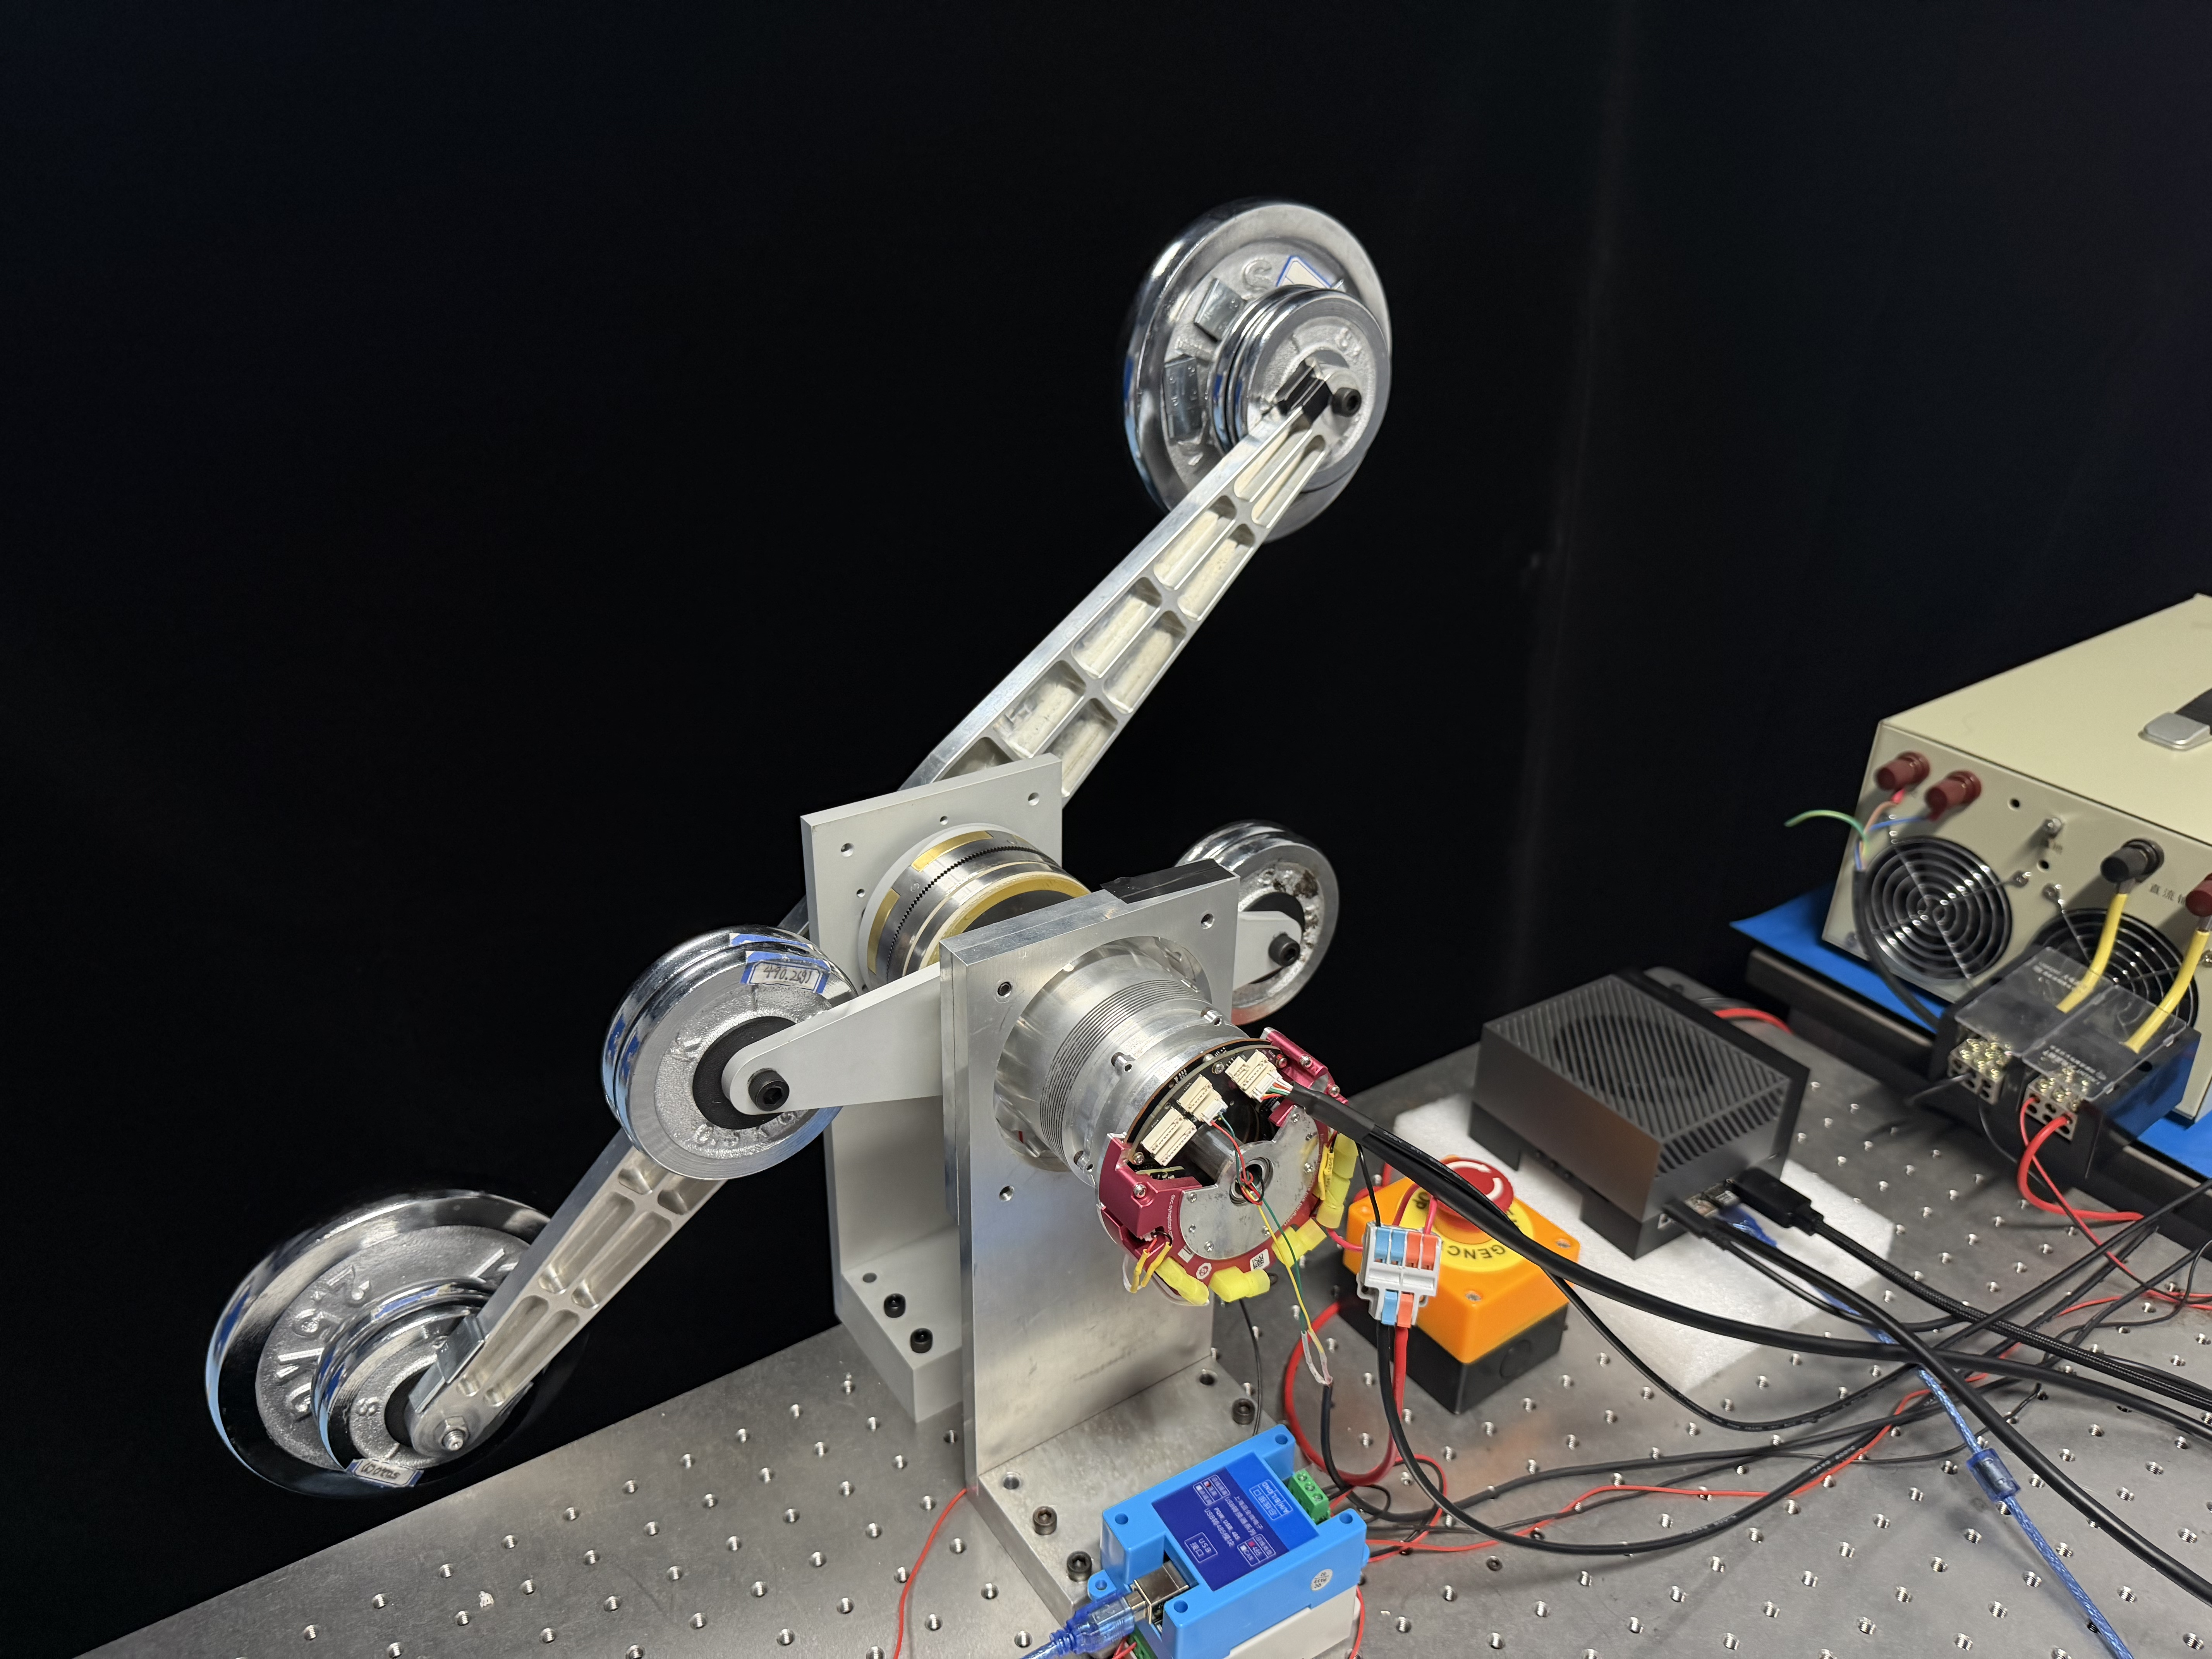
\includegraphics[width=\columnwidth]{figs/figxExam.jpg}
\caption{Photograph of the experimental SEA testbench. The platform consists of the custom SEA joint, electromagnetic clutch, and detachable rod-weight module used for variable-inertia experiments.}
\label{fig:experimental_testbench}
\end{figure}

\subsection{SEA Joint Mechanical Design}

The SEA joint is a custom-built rotational joint driven by a Kollmorgen 5008D motor through an LCSG-25-100 reducer from Leaderdrive, with a reduction ratio of 100:1. The elastic element is installed between the motor-side transmission and the output side, enabling joint torque estimation from elastic deformation.

The external inertia module uses a symmetric long-rod structure. The distance from the rod center to each side mounting hole is 300 mm. Multiple detachable masses are available, including 500 g, 1.25 kg, and 2.5 kg weights. To match the simulation settings, two inertia configurations are currently used. For the medium-inertia state, two 500 g masses are mounted symmetrically on each side; together with the long rod and the small end mounting rods, the equivalent engaged inertia is approximately 0.3 kg$\cdot$m$^2$. For the high-inertia state, each side is equipped with two 500 g masses and one 2.5 kg mass, resulting in an equivalent engaged inertia of approximately 0.75 kg$\cdot$m$^2$. Other inertia values can be obtained by changing the mass combination and mounting position.

\subsection{Sensing and Actuation}

The joint is instrumented with three 20-bit encoders: a motor-side encoder, an output-side encoder, and an elastic-element deformation encoder. The motor-side and output-side encoders provide the relative motion of the SEA two-inertia system, while the deformation encoder directly measures the elastic deflection used for torque-related feedback. The motor drive provides current control and built-in protection functions, including over-current, over-temperature, and over-torque protection.

\subsection{Hardware-Oriented Friction Profile}

The fixed high-friction simulation benchmark in Table~\ref{tab:system_params} is retained unchanged for algorithm comparison. Deployment-oriented retraining instead uses parameters identified from the physical joint and a Stribeck model
\begin{equation}
\tau_f(v)=\left[F_c+(F_s-F_c)e^{-(|v|/v_s)^2}\right]\tanh(v/\epsilon)+Bv,
\label{eq:hardware_stribeck}
\end{equation}
which separates breakaway friction $F_s$ from steady-motion Coulomb friction $F_c$. The nominal motor-side values are $F_c=2.72$~N$\cdot$m, $F_s=4.70$~N$\cdot$m, and $B=9.26$~N$\cdot$m$\cdot$s/rad; the corresponding load-side values are 0.85~N$\cdot$m, 0.85~N$\cdot$m, and 1.93~N$\cdot$m$\cdot$s/rad. The measured spring stiffness is 2400~N$\cdot$m/rad.

For hardware-oriented teacher and student training, the independently sampled ranges are $F_{c,m}\in[2.0,3.8]$, $F_{s,m}\in[4.0,7.5]$, $B_m\in[4.0,12.0]$, $F_{c,l}\in[0.5,1.2]$, $F_{s,l}\in[0.6,1.4]$, and $B_l\in[0.3,5.5]$ in consistent SI units, with $F_s\geq F_c$. We further randomize $v_s\in[0.02,0.08]$~rad/s, $\epsilon\in[0.005,0.02]$~rad/s, direction-dependent multipliers in $[0.85,1.15]$, and stiffness deviation in $[-120,120]$~N$\cdot$m/rad. The dynamic-friction split was recalculated from joint-level measurements but has not yet been independently revalidated with the final stiffness; the breakaway split is approximate. These values therefore define a deployment-training domain rather than new parameters for the simulation comparison.

\subsection{Control and Computing Hardware}

The real-time controller is an NVIDIA Jetson Orin control box running a real-time Linux kernel. The joint drive and sensor interface communicate with the controller through a 200 Hz EtherCAT loop. The trained TRACE policy is exported to a lightweight ONNX deployment graph and executed on the Orin controller. The electromagnetic clutch is controlled through a USB-to-RS485 relay module, allowing software-timed engagement and disengagement.

\subsection{Variable-Inertia Mechanism}

The clutch-based design implements a repeatable hybrid inertia transition. In the disengaged state, the joint output is connected only to the internal base inertia, producing the low-inertia condition $J_l \approx 0.05$ kg$\cdot$m$^2$. In the engaged state, the external rod-weight module is rigidly coupled to the joint, and the load inertia becomes
\begin{equation}
J_l = J_{\text{base}} + J_{\text{rod}} + \sum_i m_i r_i^2 + J_{\text{mount}},
\label{eq:testbench_inertia}
\end{equation}
where $J_{\text{base}}$ is the internal base inertia, $J_{\text{rod}}$ is the rod inertia, $m_i$ and $r_i$ are the mounted mass and its distance from the rotation axis, and $J_{\text{mount}}$ accounts for the small end mounting rods and fixtures. The symmetric mass layout reduces static imbalance and allows the target inertia to be changed by replacing the end weights while the clutch is disengaged.

\subsection{Experimental Protocol}

The hardware protocol is designed to reproduce the payload release and payload attachment process. At the beginning of an experiment, the clutch is engaged with the external inertia module configured to approximately 0.3 kg$\cdot$m$^2$. At $t=3$ s, the Orin controller sends a disengagement command through the USB-to-RS485 relay, decoupling the external module and reducing the connected inertia to the 0.05 kg$\cdot$m$^2$ base inertia. During the disengaged interval from 3 s to 10 s, the external rod is reconfigured by adding the 2.5 kg masses. At $t=10$ s, the controller sends an engagement command, coupling the high-inertia configuration of approximately 0.75 kg$\cdot$m$^2$ back to the joint. If a timing sequence identical to the simulation benchmark is required, the second engagement command can be issued at $t=7$ s after the mass reconfiguration is completed.

\subsection{Planned Hardware Test Scenarios}

The hardware evaluation is designed to cover inertia transitions that correspond to realistic assistive and domestic manipulation events. The planned test scenarios are listed in Table~\ref{tab:hardware_scenarios}. In all cases, the clutch-induced inertia sequence uses the same physical levels as the simulation benchmark, namely $0.3 \rightarrow 0.05 \rightarrow 0.75$ kg$\cdot$m$^2$, unless otherwise specified. The constant-speed test examines whether the controller can maintain smooth motion when the reflected inertia changes during continuous rotation. The sinusoidal test reproduces the simulation benchmark and evaluates tracking under periodic joint motion. The deceleration test evaluates a safety-oriented behavior in which the joint must reduce speed while the load inertia changes, corresponding to a robot slowing down after detecting a payload change or a nearby human.

\begin{table*}[t]
\centering
\caption{Planned Hardware Test Scenarios and Practical Motivations}
\label{tab:hardware_scenarios}
\footnotesize
\begin{tabular}{@{}p{0.11\textwidth}p{0.24\textwidth}p{0.22\textwidth}p{0.31\textwidth}@{}}
\toprule
Scenario & Commanded motion & Inertia transition & Practical motivation \\
\midrule
H1 & Constant-speed rotation & $0.3 \rightarrow 0.05 \rightarrow 0.75$ kg$\cdot$m$^2$ & A robot joint continues sweeping or transporting an object while a payload is released and then a heavier object is attached. \\
H2 & Sinusoidal tracking, $A=0.5$ rad, $f=0.3$ Hz & $0.3 \rightarrow 0.05 \rightarrow 0.75$ kg$\cdot$m$^2$ & A periodic assistive or manipulation motion experiences object pick-up, release, or re-grasping during operation. \\
H3 & Decelerating motion during inertia transition & $0.3 \rightarrow 0.05$ or $0.05 \rightarrow 0.75$ kg$\cdot$m$^2$ & A service or companion robot intentionally slows down after detecting load change, object slip, or close human interaction. \\
H4 & Fixed-inertia sinusoidal tracking & $0.3$ and $0.75$ kg$\cdot$m$^2$ separately & Baseline verification that the controller remains accurate and stable without a switching event. \\
\bottomrule
\end{tabular}
\end{table*}

For each scenario, the recorded signals will include reference and measured joint positions, motor-side and output-side velocities, elastic deflection, commanded and measured torque/current, normalized policy action, estimated inertia, configured inertia state, clutch command timing, inference time, and control-loop period. The main evaluation metrics are tracking RMSE, maximum tracking error, torque RMS, saturation rate, post-transition recovery time, and inertia-estimation transient behavior.

\subsection{Sim-to-Real Transfer}

The deployed controller uses the same 9-D measurable observation structure as the simulation policy, including motor-side tracking error, output-side tracking error, elastic deflection, reference trajectory, and previous action. During hardware-oriented retraining only, the privileged teacher context is expanded to represent the Stribeck and direction-asymmetry parameters in~\eqref{eq:hardware_stribeck}; these quantities are not inputs to the deployed student. The trained policy and adaptation modules are exported to ONNX for real-time execution. The ONNX result in Section~\ref{sec:computational_performance} shows that the control-only graph requires at least two CPU inference threads on the target Orin to avoid 5-ms neural-inference deadline misses in the measured run. Hardware deployment additionally requires calibration of encoder offsets, elastic-element sign convention, torque scaling, and clutch timing delay.

\subsection{Hardware Experimental Results}

Hardware experiments are in progress. The H2 sinusoidal inertia-switching test will provide the full comparison between TRACE and the simulation baselines. H1, H3, and H4 will primarily evaluate TRACE across complementary motion conditions, with conventional baselines added only where they clarify fixed-inertia or constant-speed behavior. The reported signals will quantify tracking, torque, inertia estimation, transition recovery, and the sim-to-real gap.

\section{Conclusion}

This paper presents TRACE, a timescale-resolved teacher--student controller for SEAs under abrupt load-inertia variations. A bounded dual-timescale attention branch estimates explicit inertia, while a Slow TCN Branch represents longer-context residual dynamics from non-privileged history.

In the matched zero-phase simulation, TRACE achieves 0.0140~rad RMSE under the $0.3\rightarrow0.05\rightarrow0.75$~kg$\cdot$m$^2$ transition, compared with 0.0154 for same-reward RMA, 0.0203 for PPO, 0.0248 for tuned PD+DOB, and 0.0821 for LQR. The final Fast Attention v2 estimator further achieves 0.0279~kg$\cdot$m$^2$ mean and 0.0790~kg$\cdot$m$^2$ worst stable-segment RMSE across 108 closed-loop conditions.

The final ONNX graph meets the 200~Hz inference target on Jetson Orin with two or four CPU threads, whereas one thread incurs a 1.6\% deadline-miss rate. The remaining evidence is single-DOF and simulation-led; strict component ablations and the clutch-based hardware experiments will determine how much of the observed transient benefit transfers to the physical SEA.

% Add an Acknowledgment section after funding and collaborator wording is confirmed.

\bibliographystyle{IEEEtran} 
\bibliography{references} 

% \begin{IEEEbiography}[{\includegraphics[width=1in,height=1.25in,clip,keepaspectratio]{author_photo}}]{First Author}
% Biography text here.
% \end{IEEEbiography}
%
% \begin{IEEEbiography}[{\includegraphics[width=1in,height=1.25in,clip,keepaspectratio]{author_photo}}]{Second Author}
% Biography text here.
% \end{IEEEbiography}

\end{document}
